\setchapterpreamble[u]{\margintoc}
\chapter{IP security}
\labch{chapter9}

Perché IPsec:
\begin{itemize}
    \item Il protocollo Internet (IP) non è sicuro:  è stato progettato nelle prime fasi di Internet in cui  la sicurezza non era un problema. Non garantisce integrità o riservatezza dei dati, è soggetto a replay di pacchetti e spoofing della fonte;
	\item IPsec fornisce un canale sicuro per tutte le applicazioni (cifratura e autenticazione del traffico);
	\item IPsec permette di fare un filtraggio basato su policy;
	\item È installato nei pc (per garantire sicurezza end-to-end) e gateway (firewall, router).
\end{itemize}

IPsec garantisce:
\begin{itemize}
    \item Riservatezza, cifrando i dati;
	\item Integrità, verificata dai router calcolando l'hash o il checksum del messaggio;
	\item Autenticazione, tramite firme e certificati.
\end{itemize}

Overview sulla sicurezza IP, RFC 1636:
\begin{itemize}
    \item Identifica le aree chiave per i meccanismi di sicurezza:
	\begin{itemize}
	    \item Necessità di proteggere l'infrastruttura di rete da monitoraggio e controllo non autorizzati del traffico di rete;
		\item Necessità di proteggere il traffico da utente finale a utente finale utilizzando meccanismi di autenticazione e crittografia.
	\end{itemize}
	\item Includeva l'autenticazione e la crittografia come funzionalità di sicurezza necessarie nell'IP di prossima generazione (IPv6). Ora la specifica IPsec esiste come un insieme di standard di Internet.
\end{itemize}

 Documenti di IPsec:
\begin{itemize}
    \item Architettura: copre i concetti generali, i requisiti di sicurezza, le definizioni e i meccanismi che definiscono la tecnologia IPsec;
	\item Authentication header (AS): estensione dell'header che permette di fornire autenticazione al messaggio.
	\item Encapsulation Security Payload Header (ESP): consiste di un header e un trailer (rimorchio) di incapsulazione che forniscono crittografia o una combinazione di crittografia e autenticazione;
	\item Internet Key Exchange (IKE): raccolta di documenti che descrivono gli schemi di gestione delle chiavi da utilizzare con IPsec;
	\item Algoritmi crittografici: comprende un ampio insieme di documenti che definiscono algoritmi crittografici per la crittografia, l'autenticazione dei messaggi, le funzioni pseudocasuali (PRF) e lo scambio di chiavi crittografiche;
	\item Altro: esistono numerose altre RFC relative a IPsec, tra cui quelli che si occupano della security policy.
\end{itemize}

Applicazioni di IPsec:
\begin{itemize}
    \item IPsec offre la capacità di proteggere le comunicazioni in LAN, WAN reti pubbliche e private, Internet, come:
	\begin{itemize}
	    \item Connettività sicura delle filiali su Internet (VPN su Internet o WAN pubblica);
		\item Accesso remoto sicuro su Internet (chiamata locale sicura all'ISP);
		\item Stabilire connettività Extranet e Intranet con i partner (comunicazioni sicure con altre organizzazioni);
		\item Miglioramento della sicurezza del commercio elettronico.
	\end{itemize}
	\item La caratteristica principale di IPsec è che può crittografare e/o autenticare tutto il traffico a livello IP. In questo modo tutte le applicazioni distribuite (accesso remoto, client/server, e-mail, trasferimento file, accesso Web) possono essere protette.
\end{itemize}

IPsec fornisce una serie di opzioni da scegliere per fare un'associazione di sicurezza tra due macchine:
\begin{itemize}
    \item IPsec fornisce servizi di sicurezza a livello IP consentendo a un sistema di: 
	\begin{itemize}
	    \item Selezionare i protocolli di sicurezza richiesti ;
		\item Determinare gli algoritmi da utilizzare per i servizi;
		\item Prepara le chiavi necessarie per i servizi richiesti;
	\end{itemize}
	\item RFC 4301 elenca i seguenti servizi:
	\begin{itemize}
	    \item Controllo degli accessi;
		\item Integrità senza connessione;
		\item Autenticazione sull'origine dei dati;
		\item Rifiuto dei pacchetti riprodotti/replayed (una forma di integrità parziale della sequenza);
		\item Riservatezza, tramite crittografia;
		\item Cerca di ridurre l'analisi sul traffico.
	\end{itemize}
\end{itemize}

\section{Architettura IP}

\begin{figure}[h]
    \centering
    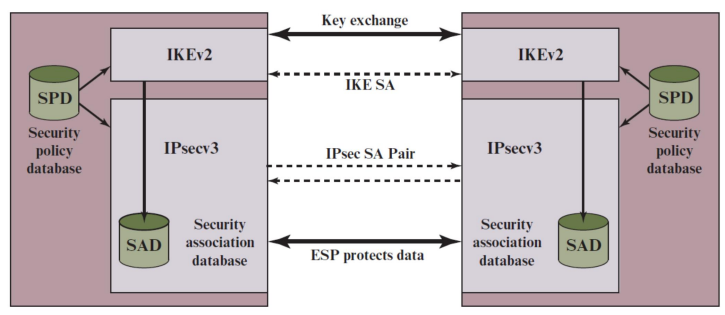
\includegraphics[width=1\textwidth]{images/chapter9/9-1.png}
    \caption{Reti wireless.}
    \label{fig:9-1}
\end{figure}

La politica IPsec è determinata dall'interazione di due database: il database dell'associazione di sicurezza (SAD) e il database della politica di sicurezza (SPD)

Security Association (SA):
\begin{itemize}
    \item Connessione logica unidirezionale tra un mittente e un destinatario che offre servizi di sicurezza sul traffico che trasporta;
	\item Nel senso inverso l'associazione di sicurezza potrebbe essere diversa;
	\item In qualsiasi pacchetto IP, la SA è identificata in modo univoco dall'indirizzo di destinazione nell'header IP e dall'SPI presente nell'estensione dell'header (AH o ESP).
\end{itemize}

Un'associazione di sicurezza è identificata da 3 parametri:
\begin{enumerate}
    \item Security Parameter Index (SPI): intero senza segno a 32 bit usatp per identificare in modo univoco questo SA e con significato solo locale (trasportato nell'intestazione IPsec: AH o ESP);
	\item Indirizzo IP di destinazione: indirizzo dell'endpoint di destinazione della SA, che può essere un sistema dell'utente finale o un sistema di rete come un firewall o un router;
	\item Identificatore del protocollo di sicurezza: indica se l'associazione è un'associazione di sicurezza AH o ESP.
\end{enumerate}

Security Association Database (SAD):
\begin{itemize}
    \item Definisce i parametri associati a ciascuna SA;
	\item Normalmente definito dai seguenti parametri in una entry SAD: 
	\begin{itemize}
	    \item Indice del parametro di sicurezza;
		\item Contatore del numero di sequenza (info sui pacchetti che seguono che hanno quell'associazione di sicurezza);
		\item Overflow del contatore di sequenza (per impedire ulteriori trasmissioni di pacchetti);
		\item Finestra anti-replay (per determinare se un pacchetto AH o ESP in entrata è un replay);
		\item Informazioni AH (algoritmo di autenticazione, chiavi, durata delle chiavi, parametro utilizzato con AH);
		\item Informazioni ESP (encr./auth. Algorithms, keys, init. values, key lives, param. ESP);
		\item Durata di questa associazione di sicurezza;
		\item Modalità del protocollo IPsec (tunnel, trasporto, wildcard);
		\item Path MTU (dimensione massima di un pacchetto che può essere trasmessa senza frammentazione).
	\end{itemize}
\end{itemize}

Security Policy Database (SPD):
\begin{itemize}
    \item Specifica le modalità attraverso le quali il traffico IP è correlato a specifiche SA. Contiene una serie di entry, ognuna delle quali definisce un sottoinsieme di traffico IP e punta a una SA per quel traffico;
	\item In ambienti più complessi, potrebbero esserci più voci che potenzialmente si riferiscono a una singola SA o a più SA associate a una singola voce SPD:
	\begin{itemize}
	    \item Ciascuna entry SPD è definita da una serie di valori di campo del protocollo IP e di livello superiore chiamati selettori;
		\item Questi sono utilizzati per filtrare il traffico in uscita al fine di mapparlo in una particolare SA.
	\end{itemize}
\end{itemize}

Una entry SPD è formata come segue:
\begin{itemize}
    \item Indirizzo IP remoto: può essere un singolo indirizzo IP, un elenco enumerato o un intervallo di indirizzi o una maschera. Gli ultimi due sono necessari per supportare più di un sistema di destinazione che condivide la stessa SA;
	\item Indirizzo IP locale: può essere un singolo indirizzo IP, un elenco enumerato o un intervallo di indirizzi o una maschera. Gli ultimi due sono richiesti per supportare più di un sistema sorgente che condivide la stessa SA;
	\item Protocollo del livello superiore: l'intestazione del protocollo IP include un campo che designa il protocollo operante su IP (TCP, UDP);
	\item Nome: un identificatore utente dal sistema operativo. Non è un campo nell'header di IP o dei protocolli superiori, ma è disponibile se IPsec è in esecuzione sullo stesso sistema operativo dell'utente;
	\item Porte locali e remote: possono essere valori di singole porte TCP o UDP, un elenco enumerato di porte o una porta con caratteri jolly.
\end{itemize}

\begin{figure}[h]
    \centering
    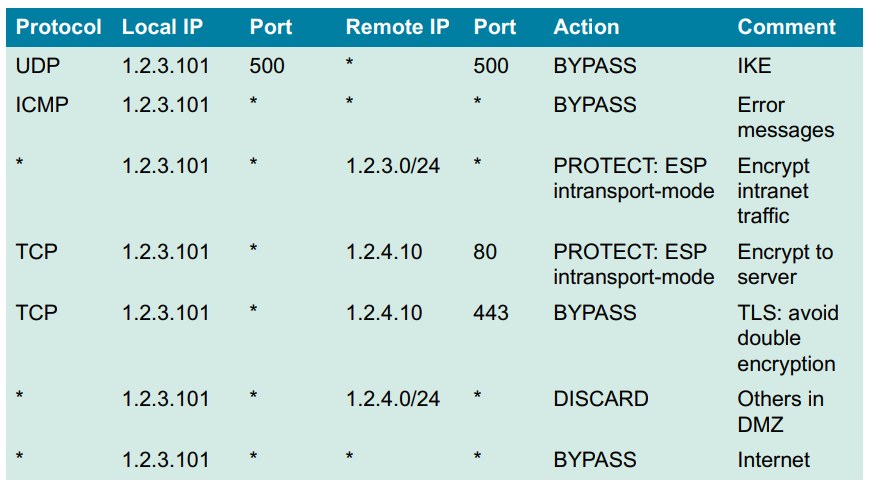
\includegraphics[width=1\textwidth]{images/chapter9/9-2.png}
    \caption{Reti wireless.}
    \label{fig:9-2}
\end{figure}

\subsection{Flow per pacchetti in entrata}

\begin{figure}[h]
    \centering
    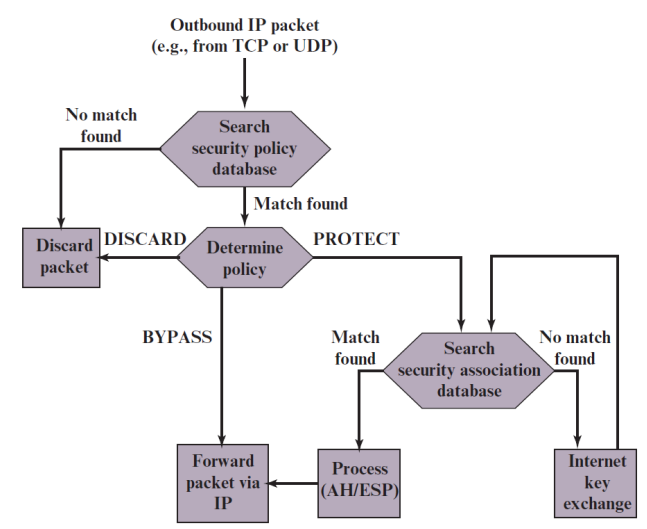
\includegraphics[width=1\textwidth]{images/chapter9/9-3.png}
    \caption{Reti wireless.}
    \label{fig:9-3}
\end{figure}

\subsection{Flow per pacchetti in uscita}

\begin{figure}[h]
    \centering
    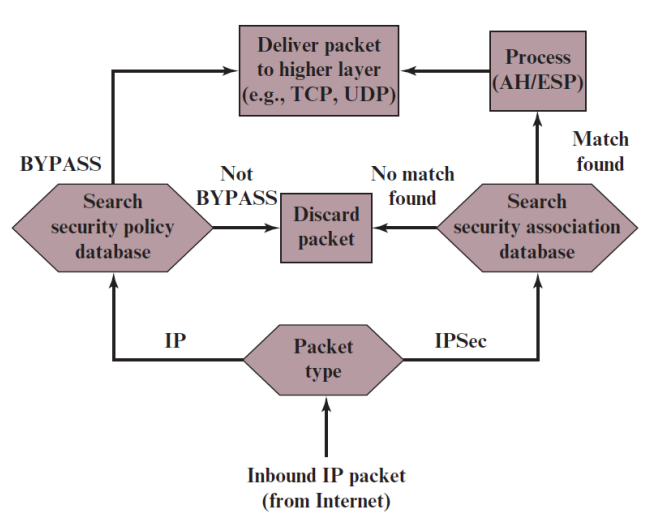
\includegraphics[width=1\textwidth]{images/chapter9/9-4.png}
    \caption{Reti wireless.}
    \label{fig:9-4}
\end{figure}

\section{Modalità di IPsec}

L'header di IPsec può essere AH o ESP.

Modalità Tunnel:
\begin{itemize}
    \item L'intero pacchetto IP viene crittografato e diventa il componente di dati di un nuovo (e più grande) pacchetto IP (il routing cambia);
	\item Utilizzato frequentemente in una VPN IPsec da sito a sito.
\end{itemize}

Modalità di trasporto:
\begin{itemize}
    \item L'header di IPsec viene inserito nel pacchetto IP (il routing rimane intatto);
	\item Non viene creato nessun nuovo pacchetto (l'header di AH assicura che gli indirizzi IP restino invariati);
	\item Funziona bene in reti in cui aumentare la dimensione del pacchetto causerebbe problemi;
	\item Utilizzato frequentemente per VPN ad accesso remoto (originariamente introdotte per permettere ai lavoratori da qualunque luogo del modo di connettersi in modo sicuro alla rete aziendale).
\end{itemize}

\begin{figure}[h]
    \centering
    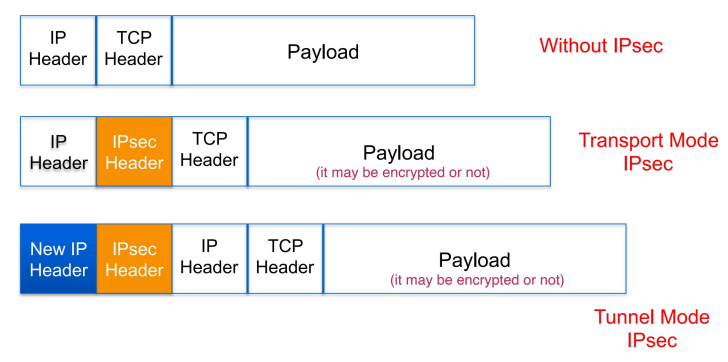
\includegraphics[width=1\textwidth]{images/chapter9/9-5.png}
    \caption{Reti wireless.}
    \label{fig:9-5}
\end{figure}

\subsection{Autentication Header (AH)}

Caratteristiche:
\begin{itemize}
    \item Header aggiuntivo tra i livelli 3 e 4 (TCP e IP) che fornisce informazioni sufficienti alla destinazione per identificare SA;
	\item AH garantisce solo l'integrità, ma protegge anche parte dell'intestazione IP;
    \item Il numero di sequenza viene inizializzato a zero e incrementato dal mittente per ogni pacchetto. Il ricevitore memorizza i pacchetti in arrivo in una finestra scorrevole (dimensione predefinita 64) per ordinare e individuare i duplicati. (IP non garantisce la consegna o l'ordine).
\end{itemize}

\begin{figure}[h]
    \centering
    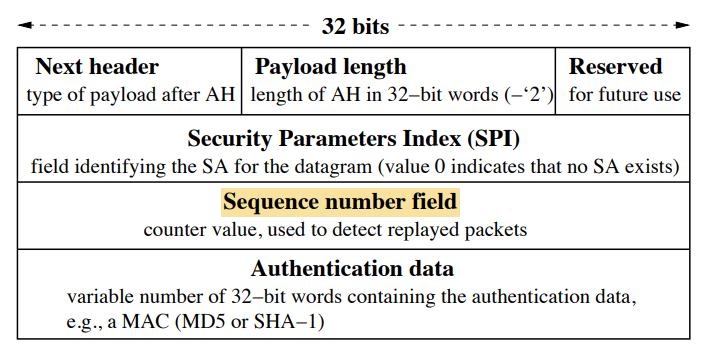
\includegraphics[width=1\textwidth]{images/chapter9/9-6.png}
    \caption{Reti wireless.}
    \label{fig:9-6}
\end{figure}

Nello specifico AH:
\begin{itemize}
    \item Per la modalità di trasporto inserisce:
	\begin{itemize}
	    \item L'intestazione IP, prima del payload IP;
		\item MAC calcolato sull'intero pacchetto (tranne che per i campi mutabili);
		\item  Fornisce protezione end-to-end tra i sistemi abilitati IPsec. 
	\end{itemize}
	\item Per la modalità tunnel:
	\begin{itemize}
	    \item L'intero pacchetto originale viene autenticato;
		\item Viene aggiunta un nuovo header IP esterno;
		\item L'header interno contiene l'indirizzo di origine/destinazione definitivo;
		\item Anche il nuovo header esterno è protetto (tranne i campi modificabili) e può contenere diversi indirizzi IP, ad esempio firewall o gateway di sicurezza.
	\end{itemize}
\end{itemize}

AH è utilizzato per fornire canali autenticati end-to-end (in genere modalità di trasporto) o nel modello di tunnel a un gateway di sicurezza.

\begin{figure}[h]
    \centering
    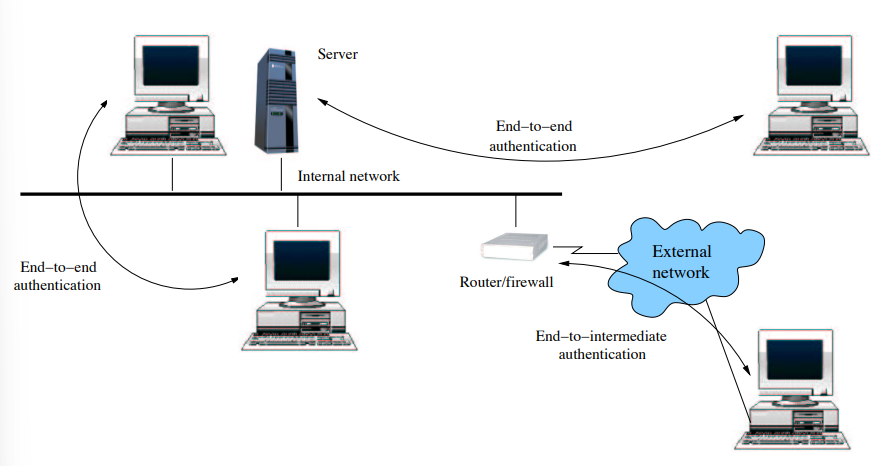
\includegraphics[width=1\textwidth]{images/chapter9/9-7.png}
    \caption{Reti wireless.}
    \label{fig:9-7}
\end{figure}

\subsection{Encapsulation Security Payload (ESP)}

Caratteristiche:
\begin{itemize}
    \item Utilizzato per crittografarei campi di payload, padding, lunghezza del padding e next header;
	\item Se l'algoritmo richiede dati di sincronizzazione per la crittografia, questi possono essere trasportati esplicitamente all'inizio del payload;
	\item Un campo ICV facoltativo è presente solo se il servizio di integrità è selezionato e fornito da un algoritmo di integrità separato o da un algoritmo in modalità combinata che utilizza un ICV:
	\begin{itemize}
	    \item L'ICV viene calcolato dopo l'esecuzione della crittografia;
		\item Questo ordine di elaborazione facilita la riduzione dell'impatto di attacchi DDoS;
		\item Poiché l'ICV non è protetto dalla crittografia, è necessario utilizzare un algoritmo di integrità con chiave per calcolare l'ICV;
	\end{itemize}
	\item Il campo relativo al padding ha più scopi:
	\begin{itemize}
	    \item Se un algoritmo di crittografia richiede che il testo in chiaro sia un multiplo di un certo numero di byte, il campo Padding viene utilizzato per espandere il testo in chiaro alla lunghezza richiesta;
		\item Viene usato per assicurare l'allineamento dei campi Pad Length e Next Header;
		\item Del padding addizionale può essere aggiunto per garantire una riservatezza parziale del flusso di traffico nascondendo la lunghezza effettiva del carico utile.
	\end{itemize}
\end{itemize}

\begin{figure}[h]
    \centering
    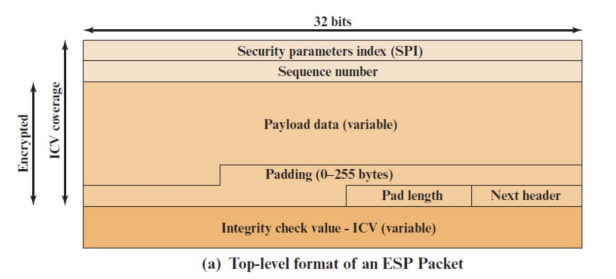
\includegraphics[width=1\textwidth]{images/chapter9/9-8.png}
    \caption{Reti wireless.}
    \label{fig:9-8}
\end{figure}

\begin{figure}[h]
    \centering
    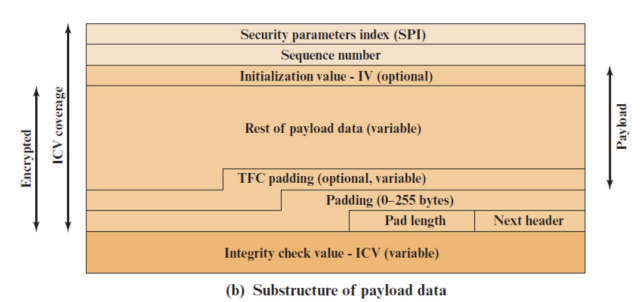
\includegraphics[width=1\textwidth]{images/chapter9/9-9.png}
    \caption{Reti wireless.}
    \label{fig:9-9}
\end{figure}

Nello specifico:
\begin{itemize}
    \item L'header specifica la crittografia e l'autenticazione. Quest'ultima è opzionale;
	\item Per la modalità di trasporto crittografa solo la parte di dati (carico utile) di ciascun pacchetto e lascia intoccato l'header;
	\item Per la modalità tunnel l'intero datagramma IP viene incapsulato all'interno dell'ESP. Il nuovo header può contenere indirizzi IP differenti (es: gateway di sicurezza). Il vecchio header e il payload vengono cifrati (e opzionalmente autenticati).
\end{itemize}

\section{Meccanismo per l'anti-replay}

Poiché la ricezione di pacchetti IP duplicati e autenticati può interrompere il servizio; il numero di sequenza viene usato per sviare questo tipo di attacchi:
\begin{itemize}
    \item Quando viene stabilito un nuovo SA, il mittente inizializza un contatore del numero di sequenza su 0, che viene incrementato ogni volta che un pacchetto viene inviato su questa SA;
	\item IP è senza connessione; non garantisce la consegna e la consegna in ordine;
	\item Il ricevitore implementa una finestra di dimensione W:
	\begin{itemize}
	    \item Se il pacchetto ricevuto cade nella finestra, viene controllato il MAC e se autenticato viene contrassegnato il suo slot ;
		\item Se il pacchetto ricevuto è sulla destra della finestra, vengono controllati MAC e auth e, se passati, la finestra viene spostata a destra;
		\item Se il pacchetto ricevuto è a sinistra o l'autenticazione non riesce, il pacchetto viene scartato.
	\end{itemize}
\end{itemize}

\begin{figure}[h]
    \centering
    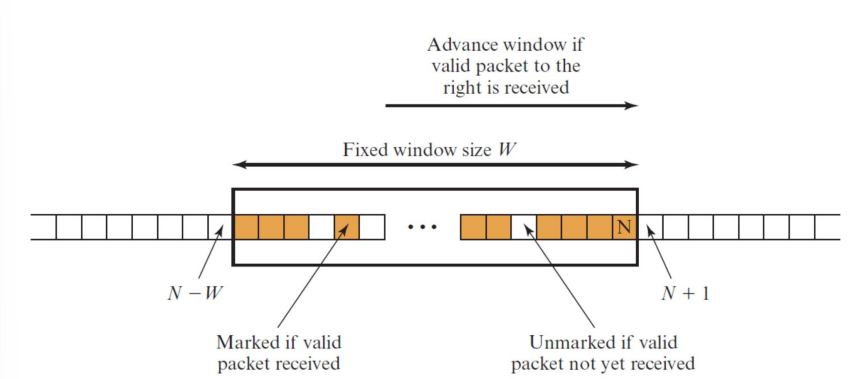
\includegraphics[width=1\textwidth]{images/chapter9/9-10.png}
    \caption{Reti wireless.}
    \label{fig:9-10}
\end{figure}

Modalità di trasporto per ESP

Funzionamemto:
	\item Alla fonte, il blocco di dati costituito dal trailer ESP più l'intero segmento del livello di trasporto viene crittografato e il testo in chiaro di questo blocco viene sostituito con il suo testo cifrato per formare il pacchetto IP per la trasmissione. L'autenticazione viene aggiunta se questa opzione è selezionata;
	\item Il pacchetto viene quindi instradato alla destinazione. Ogni router intermedio deve esaminare ed elaborare l'header IP più qualsiasi header di estensione IP in chiaro ma non ha bisogno di esaminare il testo cifrato;
	\item Il nodo di destinazione esamina ed elabora l'IP header più eventuali intestazioni di estensione IP in chiaro. Quindi, sulla base dell'SPI nell'intestazione ESP, il nodo di destinazione decrittografa il resto del pacchetto per recuperare il segmento del livello di trasporto in plain-text.
	
Il funzionamento in modalità trasporto garantisce la riservatezza per qualsiasi applicazione che lo utilizzi, evitando così la necessità di implementare la riservatezza in ogni singola applicazione. Uno svantaggio di questa modalità è che è possibile fare analisi del traffico  sui pacchetti trasmessi.

\subsection{Modalità tunnel}

La modalità Tunnel fornisce protezione al pacchetto IP:
\begin{enumerate}
    \item Per ottenere ciò, dopo aver aggiunto i campi AH o ESP al pacchetto IP, l'intero pacchetto più i campi di sicurezza vengono trattati come il payload del nuovo pacchetto IP esterno con un nuovo header IP esterno;
	2. L'intero pacchetto originale, ora interno, viaggia attraverso un tunnel da un punto all'altro di una rete IP; nessun router lungo il percorso è in grado di esaminare l'header IP interno;
	3. Poiché il pacchetto originale è incapsulato, il nuovo pacchetto più grande potrebbe avere indirizzi di origine e destinazione completamente diversi, aumentando la sicurezza;
\end{enumerate}

Caratteristiche:
\begin{itemize}
    \item La modalità Tunnel viene utilizzata quando una o entrambe le estremità della Security Association (SA) sono un gateway di sicurezza, come un firewall o un router che implementa IPsec;
	\item Con la modalità tunnel, gli host sulle reti dietro i firewall possono impegnarsi in comunicazioni sicure senza implementare Ipsec;
	\item I pacchetti non protetti generati da tali host vengono incanalati attraverso reti esterne tramite la modalità tunnel, come impostato dal software IPsec nel firewall o nel router sicuro al confine della rete locale.
	\item La modalità tunnel è utile in una configurazione che include un firewall o un altro tipo di gateway di sicurezza che protegge una rete affidabile da reti esterne;
	\item La crittografia avviene solo tra un host esterno e il gateway di sicurezza o tra due gateway di sicurezza:
	\begin{itemize}
	    \item Alleggerisce gli host sulla rete interna dall'elaborazione del carico di cifrare e semplifica l'attività di distribuzione delle chiavi riducendo il numero di chiavi necessarie;
		\item Contrasta l'analisi del traffico basata sulla destinazione finale.
	\end{itemize}
\end{itemize}

\section{Virtual Private Network (VPN)}

La modalità Tunnel può essere utilizzata per implementare una VPN. Una VPN è una rete privata configurata all'interno di una rete pubblica per sfruttare le economie di scala e le strutture di gestione delle grandi reti.

Vantaggi:
\begin{itemize}
    \item Le VPN sono ampiamente utilizzate dalle aziende per creare reti che si estendono su vaste aree geografiche, per fornire connessioni da sito a sito alle filiali e per consentire agli utenti mobili di collegarsi alle LAN aziendali;
	\item La struttura della rete pubblica è condivisa da molti clienti, con il traffico di ciascun cliente separato dall'altro traffico;
	\item Il traffico designato come traffico VPN può passare solo da una VPN sorgente verso una destinazione nella stessa VPN;
	\item Solitamente sono forniti crittografia e autenticazione per le VPN.
\end{itemize}

\begin{figure}[h]
    \centering
    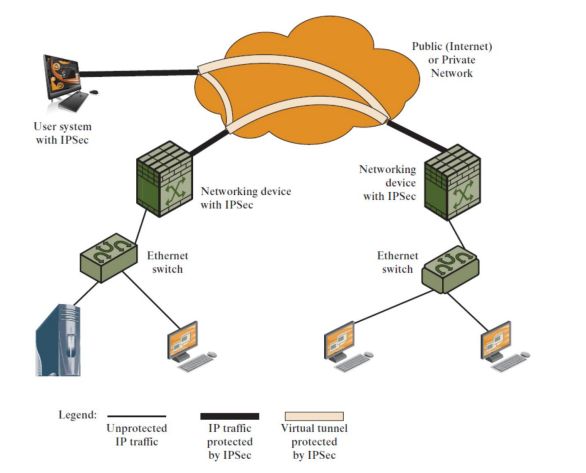
\includegraphics[width=1\textwidth]{images/chapter9/9-11.png}
    \caption{Reti wireless.}
    \label{fig:9-11}
\end{figure}

\section{Riassunto}

\begin{table}[h]
    \centering
    \begin{tabular}{ |p{0.5\textwidth}|p{0.5\textwidth}|p{0.5\textwidth}| }
         \hline
          & Modalità di trasporto SA & Modalità tunnel SA \\ 
         AH & Autentica il payload IP e porzioni selezionate dell'intestazione IP e delle intestazioni dell'estensione IPv6. & Autentica l'intero pacchetto IP interno (header interno più payload IP) più porzioni selezionate dell'header esterno IP e dell'estensione esterna di IPv6 \\ 
         ESP & Crittografa il payload IP e qualsiasi header di estensione IPv6 che segue l'header ESP. & Crittografa l'intero pacchetto IP interno. \\ 
         ESP con autenticazione & Crittografa il payload IP e qualsiasi intestazione di estensione IPv6 dopo l'header ESP. Autentica il payload IP ma non l'header IP.& Crittografa l'intero pacchetto IP interno. Autentica il pacchetto IP interno. \\ 
         \hline
    \end{tabular}
    \caption{Riassunto.}
    \label{tab:table9-1}
\end{table}

\section{Internet Key Exchange}

La parte di gestione chiave di IPsec comporta la determinazione e distribuzione delle chiavi segrete. Un requisito tipico sono quattro chiavi per la comunicazione tra due applicazioni (una coppià per integrità e una per crittografia/riservatezza).

Il documento IPsec Architecture richiede il supporto per due tipi di gestione delle chiavi:
\begin{itemize}
    \item Manuale: un amministratore di sistema configura manualmente ogni sistema con le proprie chiavi e con le chiavi di altri sistemi comunicanti (pratico per ambienti piccoli e statici);
	\item Automatizzato: consente la creazione on-demand di chiavi per SA e facilita l'utilizzo delle chiavi in un grande sistema distribuito con una configurazione in evoluzione.
\end{itemize}

\subsection{Overview}

\begin{figure}[h]
    \centering
    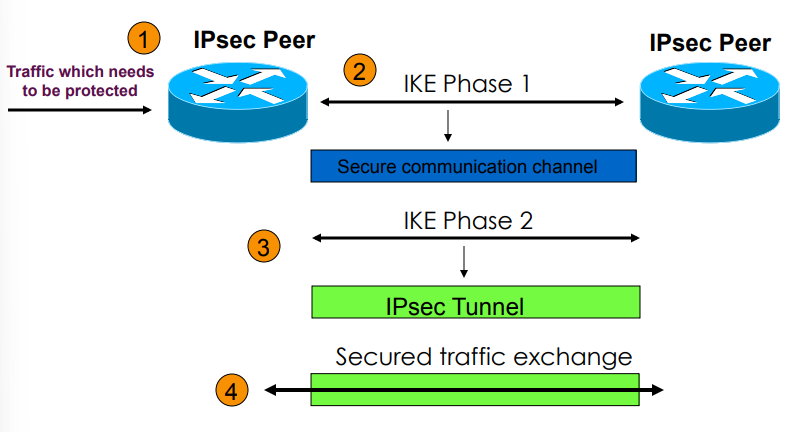
\includegraphics[width=1\textwidth]{images/chapter9/9-12.png}
    \caption{Reti wireless.}
    \label{fig:9-12}
\end{figure}

La creazione del canale può avvenire in due modi:
\begin{itemize}
    \item Main mode: i due peer non si conoscono e devono creare una canale sicuro di comunicazione. Una volta stabiliti i segreti e creato il canale, questo può essere usato epr scambiarsi altri segreti e creare sottocanali;
	\item Quick mode: usata per creare canali figli. 
\end{itemize}

Se un canale main o figlio viene compromesso, gli altri sono comunque sicuri.

\subsection{Main mode/Fase 1}

\begin{figure}[h]
    \centering
    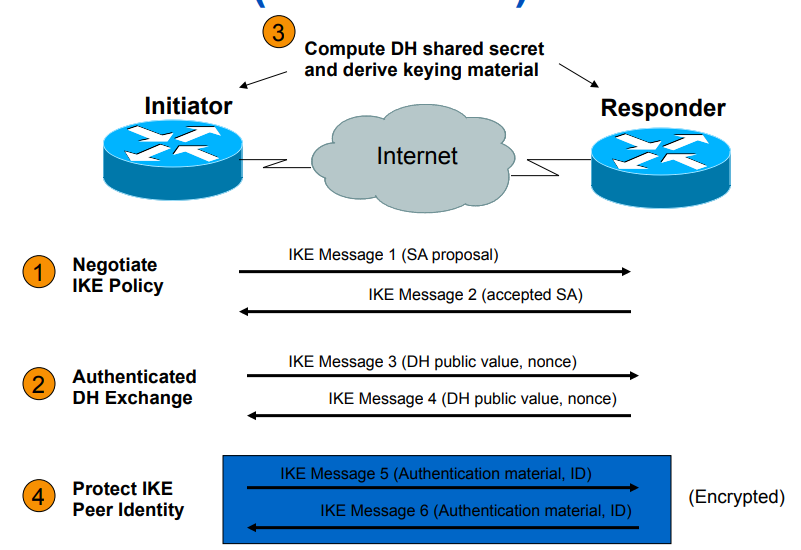
\includegraphics[width=1\textwidth]{images/chapter9/9-13.png}
    \caption{Reti wireless.}
    \label{fig:9-13}
\end{figure}

Vengono scambiati sei messaggi, a coppie di due:
\begin{enumerate}
    \item L'initiator invia una serie di proposte e un elenco di algoritmi per ogni per ogni proposta. Il responder risponde con le proposte accettate e l'algoritmo scelto per ogni proposta;
	\item Scambio autenticato delle mezze chiavi di DH e dei nonce;
	\item Scambio dell'hash crittografato della propria identità e dei messaggi scambiati, con seguente confronto.
\end{enumerate}

\subsection{ISAKMP/Oakley}

Protocollo di gestione delle chiavi automatizzato predefinito di Ipsec.

Si compone di:
\begin{itemize}
    \item  Oakley Key Determination Protocol:
	\begin{itemize}
	    \item Protocollo di scambio di chiavi basato sull'algoritmo Diffie-Hellman ma che fornisce una maggiore sicurezza;
		\item Generico in quanto non detta formati specifici
	\end{itemize}
	\item Internet Security Association and Key Management Protocol (ISAKMP):
	\begin{itemize}
	    \item Fornisce un framework per la gestione delle chiavi Internet e fornisce il supporto per il  protocollo specifico, inclusi i formati, per la negoziazione degli attributi di sicurezza;
		\item Consiste in un insieme di tipi di messaggi che consentono l'uso di una varietà di algoritmi di scambio di chiavi.
	\end{itemize}
\end{itemize}

IKE è caratterizzato da cinque caratteristiche importanti:
\begin{itemize}
    \item Impiega un meccanismo noto come cookie per contrastare attacchi di intasamento;
	\item Consente alle due parti di negoziare un gruppo; questo, in sostanza, specifica i parametri globali dello scambio di chiavi Diffie-Hellman;
	\item Usa i nonce per proteggersi dai replay attack;
	\item Consente lo scambio delle chiavi pubbliche di DF;
	\item Autentica lo scambio Diffie-Hellman per contrastare gli attacchi man-in-the-middle.
\end{itemize}

\begin{figure}[h]
    \centering
    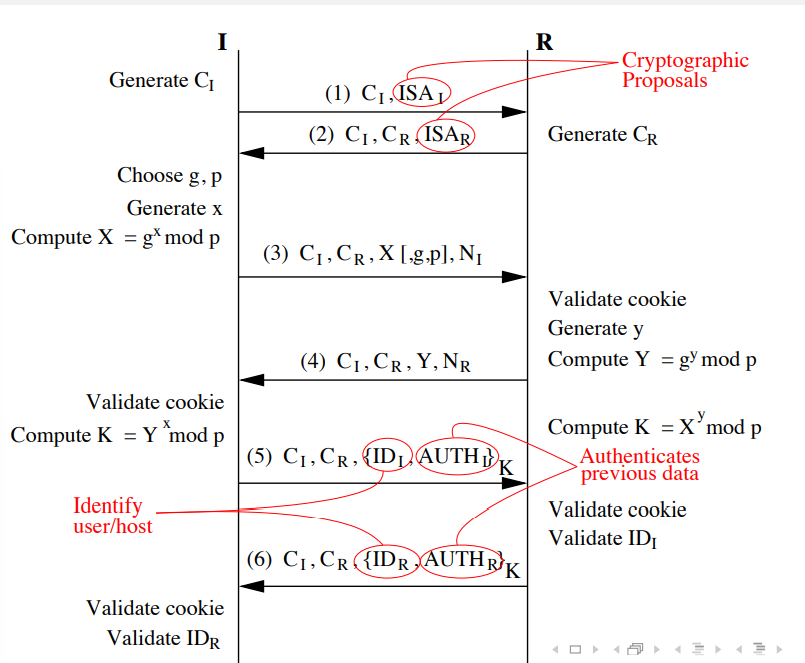
\includegraphics[width=1\textwidth]{images/chapter9/9-14.png}
    \caption{Reti wireless.}
    \label{fig:9-14}
\end{figure}

Quick mode/Fase 2

Tutto il traffico è cifrato usando ISAKMP Security Association. Ciascuna negoziazione in modalità rapida risulta in due IPsec Security Association, una in entrata e una in uscita. Vengono create/aggiornate le chiavi necessarie. 
Si può fare subito il DF autenticato facendo viaggiare il messaggio con un hash storico (il secondo messaggio viaggia con l'hash del primo e del secondo) generato dalla Master Key scambiata nella fase 1. Nei nuovi canali è possibile cambiare i parametri.

\begin{figure}[h]
    \centering
    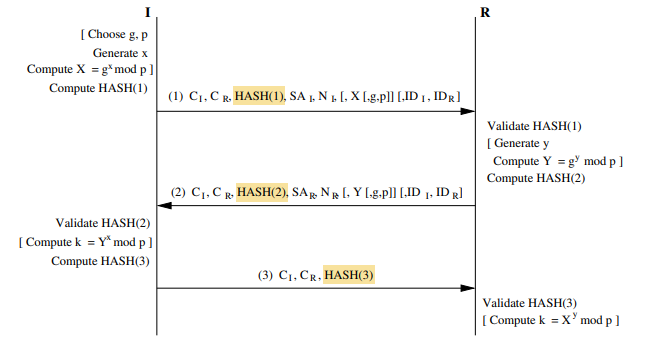
\includegraphics[width=1\textwidth]{images/chapter9/9-15.png}
    \caption{Reti wireless.}
    \label{fig:9-15}
\end{figure}

\begin{figure}[h]
    \centering
    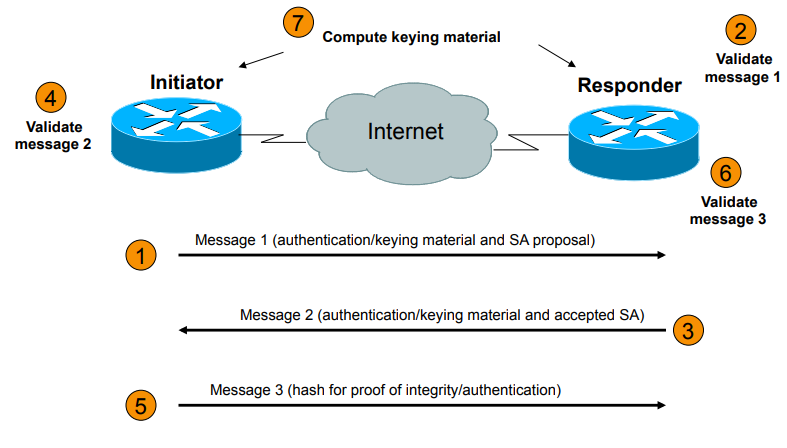
\includegraphics[width=1\textwidth]{images/chapter9/9-16.png}
    \caption{Reti wireless.}
    \label{fig:9-16}
\end{figure}

\section{Combinazione di associazioni di sicurezza }

Una singola SA può implementare il protocollo AH o ESP, ma non entramb.

Security Association bundle:
\begin{itemize}
    \item Si riferisce a una sequenza di SA attraverso le quali deve essere elaborato il traffico per fornire l'insieme di servizi IPsec desiderato;
	\item Le SA in un bundle possono terminare a diversi endpoint o allo stesso punto finale.
\end{itemize}

I bundle possono essere creati in due modi:
\begin{itemize}
    \item Adiacenze di trasporto:
	\begin{itemize}
	    \item Si riferisce all'applicazione di più di un protocollo di sicurezza allo stesso pacchetto IP senza invocare il tunneling;
		\item Questo approccio consente un solo livello di combinazione;
	\end{itemize}
	\item Tunneling iterato:
	\begin{itemize}
	    \item Si riferisce all'applicazione di più livelli di protocolli di sicurezza effettuati tramite il tunneling IP;
		\item Questo approccio consente più livelli di nidificazione.
	\end{itemize}
\end{itemize}

\section{ESP con opzione di autenticazione}

In questo approccio, il primo utente applica ESP ai dati da proteggere e poi aggiunge il campo di autenticazione dei dati. 

Varia in base alla modalità:
\begin{itemize}
    \item Modalità di trasporto ESP: l'autenticazione e la crittografia si applicano al payload IP consegnato all'host, ma l'intestazione IP non è protetta;
	\item Modalità tunnel ESP: l'autenticazione si applica all'intero pacchetto IP consegnato all'indirizzo IP di destinazione esterno e l'autenticazione viene eseguita a quella destinazione. L'intero pacchetto IP interno è protetto dal meccanismo di privacy per la consegna alla destinazione IP interna.
\end{itemize}

In entrambi i casi l'autenticazione si applica al testo cifrato anziché al testo in chiaro.

\section{Adiacenze dei trasporti}

Un altro modo per applicare l'autenticazione dopo la crittografia consiste nell'usare due SA di trasporto in bundle, con all'interno un ESP SA e all'esterno un AH SA:
\begin{itemize}
    \item In questo caso l'ESP viene utilizzato senza la sua opzione di autenticazione;
	\item La crittografia viene applicata al payload IP;
	\item AH viene quindi applicato in modalità di trasporto;
	\item Il vantaggio di questo approccio è che l'autenticazione copre più campi;
	\item Lo svantaggio è l'overhead di due SA contro una SA.
\end{itemize}

\section{Transport-Tunnel Bundle}

L'uso dell'autenticazione prima della crittografia potrebbe essere preferibile per diversi motivi:
\begin{itemize}
    \item È impossibile per chiunque intercettare il messaggio e alterare i dati di autenticazione senza essere scoperti;
	\item Potrebbe essere opportuno memorizzare le informazioni di autenticazione con il messaggio alla destinazione per riferimenti futuri.
\end{itemize}

Un approccio consiste nell'utilizzare un bundle costituito da un trasporto AH interno SA e un tunnel ESP esterno SA:
\begin{itemize}
    \item L'autenticazione viene applicata al payload IP e all'header IP;
	\item Il pacchetto IP risultante viene quindi elaborato in modalità tunnel da ESP;
	\item Il risultato è che l'intero pacchetto interno autenticato viene crittografato e viene aggiunta una nuova intestazione IP esterna.
\end{itemize}






